\chapter{Anomaly Detection Using Recurrent Neural Networks}
\label{ch:results}


\section{Introduction}

Chapters \ref{ch:ad} and \ref{ch:rnn}, separately, introduced anomaly detection in time series and recurrent neural networks as time series modelers.
%
This chapter outlines and tests a procedure for finding anomalies using RNNs with the goal of mitigating many of the problems associated with anomaly detection that were discussed in Chapters \ref{ch:ad} and \ref{ch:adtechnique}.
%
As much as possible, the same procedure is applied to each test time series to test the procedure's generality.


The procedure outline describes:
%
\begin{description}
%
\item[sampling:] the time series used for training and its associated sampling process
%
\item[recurrent autoencoders:] the specific form of the RNN
%
\item[training:] the training algorithm used on the RNN
%
\item[Bayesian optimization:] the search for optimized parameters for the procedure
%
\end{description}
%
After describing the procedure, the anomaly scores of the test time series are evaluated for their ability to detect anomalies.


\section{Sampling: Sliding Windows}
\label{sec:sampling}


Some univariate time series \emph{with} anomalies were chosen or generated to test the anomaly detection process named as follws:

\begin{description}

\item[spike:] two generated sequences that are simply evenly-spaced `spikes' of the same height.

\item[sine:] a generated sinusoidal signal.

\item[power demand:] a building's electrical power usage data%
\footnote{\url{http://www.cs.ucr.edu/~eamonn/discords/power_data.txt}} referenced in the influencial HOT-SAX paper \cite{Keogh2005} (for anomaly detection in time series). The data was scaled down by dividing it by its median (to help in the training process).

\item[electrocardiogram  (ECG):] a signal from the human heart taken from the PhysioNet \cite{PhysioNet} database. Finding anomalies in ECG data has been used as a benchmark in several studies at least \cite{Malhotra2015,Keogh2005,Cheboli2010,li2012dimensionality,Wei2005,Chuah2007,Jones2014}.

\item[polysomnography ECG (PSG-ECG):] human ECG data \cite{PhysioNet} taken during a sleep study%
\footnote{University College Dublin Sleep Apnea Database, \url{http://www.physionet.org/physiobank/database/ucddb/}, doi:10.13026/C26C7D, study id. ucddb002}%
.


\end{description}
\noindent
%
The normal behaviour, as well as anomalous behaviour, of these time series can be seen in the plots presented in Section \ref{sec:results}.%
%todo: along with an explanation of why it was chosen

While there is only one `source' time series to train on (in each test), the RNN needs to see many `samples' from the source time series.
%
The sliding window procedure, described in Section \ref{sec:adsample}, is used to get samples of some window width.
%
Additionally, since RNNs do not need a fixed window, sliding windows are obtained for more than one window width.
%
Furthermore, the samples are collected into `mini-batches' (of the same window width) to be more compatible with the training procedure.
%
The window width is incremented (width skip) from some minimum until it is not possible to obtain a mini-batch (so the largest window will be close to the length of the time series).


Table \ref{tbl:winspec} specifies the relevent sizes and increments for the sampling process.
%
The values were adjusted manually until a `reasonable' number of samples were found.
%
However, the minimum window length was chosen such that meaningful dynamics were captured (regardless of the scale of the anomaly).

%todo: why extra line ???
\begin{table}[H]
  \centering
  \csvreader[
  % need p b/c the below \ifthenelse 'filters' make the tbl cell ugly
  tabular=|p{.75in}||c|c|c|c|c||c| 
  ,table head=
  \hline
  \bfseries series
  &  length 
  &  min. win.
  &  slide skip 
  &  width skip 
  &  batch size
  &  $\Rightarrow$ \bfseries samples 
  \\ \hline  \hline
  ,late after line=\\\hline
  ]%
  {tbls/sampling.csv}%
  {
    batch_size=\bs
    ,length=\ln
    ,min_winsize=\mw
    ,name=\nm
    ,nsamples=\ns
    ,slide_jump=\ss
    ,winsize_jump=\wss
  }%
  {
    %these act like filters. so you have to explicitly get them
    \ifthenelse{ \equal{\nm}{spikelv}}{\noindent spike-1}{}
    \ifthenelse{ \equal{\nm}{spikereg}}{\noindent spike-2}{}
    \ifthenelse{ \equal{\nm}{sin}}{\noindent sine}{}
    \ifthenelse{ \equal{\nm}{power}}{\noindent power}{}
    \ifthenelse{ \equal{\nm}{ecg}}{\noindent ECG}{}
    \ifthenelse{ \equal{\nm}{sleep}}{\noindent  PSG-ECG}{}

    & \ln & \mw & \ss & \wss & \bs & \ns
  }
\caption[]{Time series sample specifications} %todo: what case?
\label{tbl:winspec}
\end{table}


\section{RNN Setup: Autoencoder}

The RNN needs to learn what normal time series behavior is.
%
So an autoencoder is used which can learn expected behavior by setting the target, $\vc{y}$, to be the input, $\vc{x}$.
%
The loss function is the MSE (Equation \ref{eqn:mse}).
%
Furthermore, to prevent the RNN from learning trivial identity functions, Gaussian noise is added to the input where the standard deviation is equal to 0.75 times the standard deviation of the whole time series.
%
\begin{equation*}
 \tilde{\x} = \x
 + \mathcal{N}(0,(0.75\sigma_{\mathrm{std}}(\x))^2)
\end{equation*}
%
Note the comparison in the loss function is between the uncorrupted signal, $\x$, and the output from the network, $\vc{o}$, given $\x$: $L(\vc{o}(\tilde{\x}),\x)$.

With this setup, a denoising autoencoder, the data generating process, $p(\x)$, is implicitly learned \cite{Bengio2013}.


\section{Training: RMSprop}
\label{sec:training}

SGD with RMSprop \cite{Tieleman2012} for parameter updates has been demonstrated to provide results that are similar to more sophisticated second-order methods but with significantly less computational cost \cite{Dauphin}.
%
Another benefit of RMSprop is that it is designed to work with mini-batch learning.
%
Since the training data is highly redundant (from sliding windows), it is expected that computing the gradient (to update parameters) from a subset of the data (mini-batch) is more efficient than computing the gradient for all the data.


For each derivative in the gradient, RMSprop keeps an exponentially-weighted moving average of derivative magnitudes which normalizes the derivative by its root-mean-squared.
%
More specifically, the (overall) RNN training procedure is outlined in the following box.


\begin{algorithm}{Training Procedure}
\begin{algorithmic}
\STATE \STATE

\STATE \COMMENT{obtain mini-batches (as Section \ref{sec:sampling})}
\STATE $\mathcal{X} \gets \mathrm{sampling}(\x)$
\STATE \STATE

\STATE \COMMENT{randomly split mini-batches into training and validation sets}
\STATE $\mathcal{X}_t \gets \mathrm{choose(75\%,\mathcal{X})}$
\STATE $\mathcal{X}_v \gets \mathcal{X} - \mathcal{X}_t$
\STATE \STATE


\STATE \COMMENT{initialize}
\STATE $\vc{\theta} \gets \vc{0}$
\COMMENT{initial RNN parameters are 0}
\STATE \COMMENT{set training parameters}
\STATE $\alpha = 10^{-4}$
\COMMENT{learning rate}
\STATE $h = 14$
\COMMENT {RMS `halflife'}
\STATE $\gamma \gets e^{\frac{-\ln{2}}{h}}$
\STATE $r = 10^{-8}$
\COMMENT{RMS regularizer}
\STATE patience = 5
\COMMENT{stopping criterion parameter}
\STATE min\_improvement = $.005$
\COMMENT{stopping criterion parameter}
\STATE \STATE

%\STATE $i \gets 1$
\FOR{epoch $i$}
\STATE{ $\mathcal{X}_t \gets  \mathrm{shuffle}(\mathcal{X}_t)$}

\FOR{mini-batch $M$ in $\mathcal{X}_t$ }

\FOR{parameter $p$ in $\vc{\theta}$}
\STATE{} \COMMENT{per-parameter, update $p$ according to RMSprop \cite{Graves2013b}
(indices to $p$ omitted)}
\STATE{
  \begin{flalign*}
    f_{i+1}
    &\gets 
    \gamma f_i 
    +
    (1 - \gamma) 
    \frac{\partial{L}}{\partial{p}} && 
    \\
    g_{i+1}
    &\gets
    \gamma g_i
    +
    (1 - \gamma)
    \left(
      \frac{\partial{L}}{\partial{p}}
    \right)^2 && 
    \\
    p_{i+1}
    &\gets 
    p_i
    - 
    \frac{\alpha}{
      \sqrt{g_{t+1} 
        - f_{t+1}^2 
        + r}
    }
    \frac{\partial{L}}{\partial{p}} &&
  \end{flalign*}
}
\ENDFOR
\ENDFOR

\STATE \COMMENT{compute average loss on validation set}
\STATE{
  $
  v_i
  \gets
  \frac{1}{|\mathcal{X}_v|}
  \sum_{\x_v \in \mathcal{X}_v}
  L(\x_v,\vc{o})
  $
}


\STATE \COMMENT{stop when no improvement more than patience times}
\IF{
$v_{min}-v_{i}> v_{min} \cdot \mathrm{min\_improvement}$
}
\STATE{$v_{min} \gets v_i$}
\STATE{$i_{min} \gets i$}
\ENDIF

\IF{$i - i_{min} > \mathrm{patience}$}
\STATE{STOP} \COMMENT{return $\vc{\theta}$}
\ENDIF

\STATE{$i \gets i+1$}
\ENDFOR

%\STATE \STATE
\end{algorithmic}
\end{algorithm}

%todo: use s=h in lstm

The \textsf{Theanets} \cite{Johnson2015} implementation%
\footnote{With every calculation of $\vc{o}$, the RNN states are initialized to 0.}
of RNNs and RMSprop was used.
%
\textsf{Theanets} is based on the mathematical expression compiler, \texttt{Theano} \cite{Bergstra2010}.
%
Gradients were computed using \textsf{Theano}'s automatic differentiation feature instead of explicitly-defined backpropagation \cite{Rumelhart1986}.

%\section{Hyper-parameter Optimization}
%In the previous section, 

While the training procedure optimizes $\vc{\theta}$, there are other parameters that could be adjusted to minimize the loss.
%
The number of layers, $l$, and the `size' of each layer, $n$, corresponding the dimension of vector $\vc{s}$ (which equals the cell state memory dimension as well), were chosen as `hyper-parameters' for optimization in a Bayesian optimization process.
%
Bayesian optimization is suited for optimizing RNN training because
1) it tries to minimize the number of (expensive) objective function calls, which, in this case, is the training procedure, and
2) it considers the stochasticity of the function, which, in this case, the selection of training and validation data are random in addition to the training data shuffling on each epoch.


The \textsf{Spearmint} \cite{snoek2012practical} package was used to drive the hyper-parameter optimization process.
%
\textsf{Spearmint} takes a parameter search space and a maximum number of optimization iterations.
%
The process was programmed to save RNN parameters after every optimization iteration.
%
However, the process was stopped until the RNN with the minimum validation loss was subjectively able to detect anomalies%
%
\footnote{
Further optimization may have been possible with increasing RNN size but loss reduction diminished relative to the associated increase in computational expense.
}%
%
.


For every sample, Figure \ref{fig:bo} shows the results of the Bayesian optimization process and the training progress of the best network.
%
In the training progress figures, the validation and validation losses are close throughout the training process.
%
This is expected since the training and validation sets are highly redundant and perhaps the RNN, by nature, interprets them to be almost identical (invariance to translation and sequence length).
%todo: results are fine eventhough it might be underfit

%todo: spike-2 legend
\begin{figure}[!hp]
    \centering %3figs a pg. these are the gen figs
  
  \begin{subfigure}[t]{\textwidth} %hmm it's the same width as the pdf
    % todo: check the previous pdfs includegraphics
        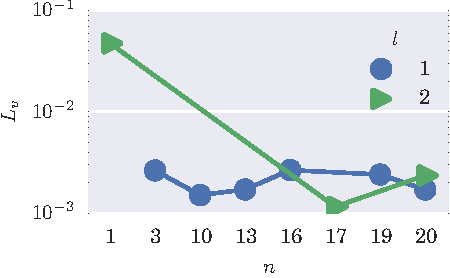
\includegraphics[width=.5\textwidth]{figs/bo_spikelv.pdf}
        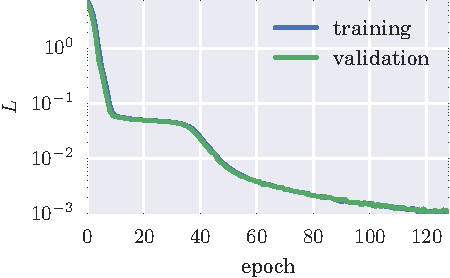
\includegraphics[width=.5\textwidth]{figs/trn_spikelv.pdf}
        \caption{spike-1}
    \end{subfigure}%

\end{figure}
\begin{figure}[!hp]
\ContinuedFloat

  \begin{subfigure}[t]{\textwidth}
        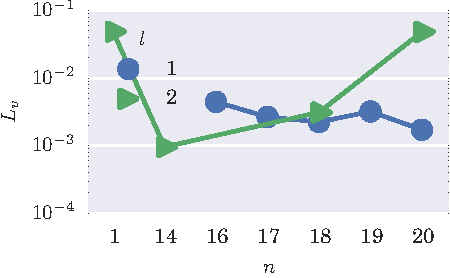
\includegraphics[width=.5\textwidth]{figs/bo_spikereg.pdf}
        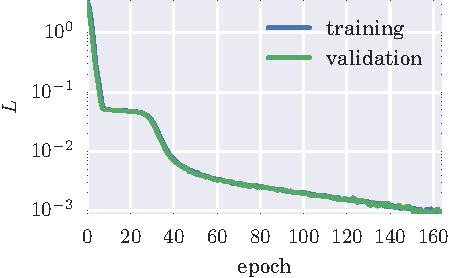
\includegraphics[width=.5\textwidth]{figs/trn_spikereg.pdf}
        \caption{spike-2}
    \end{subfigure}%

\end{figure}
\begin{figure}[!hp]
\ContinuedFloat
  
    \begin{subfigure}[t]{\textwidth}
        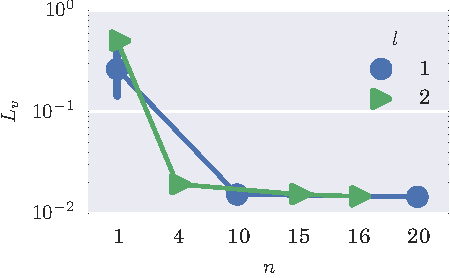
\includegraphics[width=.5\textwidth]{figs/bo_sin.pdf}
        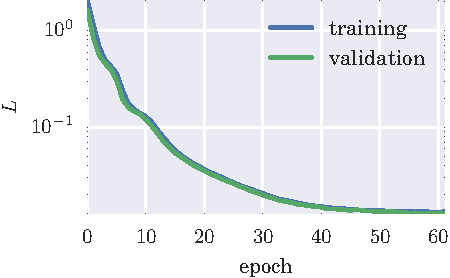
\includegraphics[width=.5\textwidth]{figs/trn_sin.pdf}
        \caption{sine}
    \end{subfigure}%

\end{figure}
\begin{figure}[!hp]
\ContinuedFloat

    \begin{subfigure}[t]{\textwidth} 
        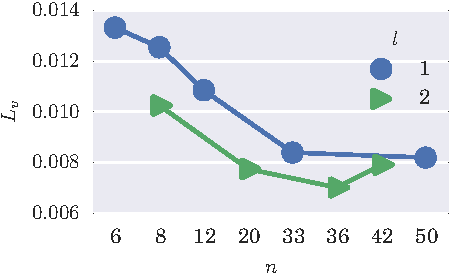
\includegraphics[width=.5\textwidth]{figs/bo_power.pdf}
        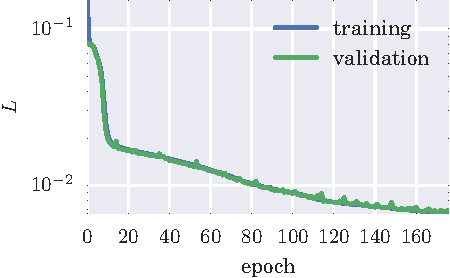
\includegraphics[width=.5\textwidth]{figs/trn_power.pdf}
        \caption{power}
    \end{subfigure}%

\end{figure}
\begin{figure}[!hp]
\ContinuedFloat

    \begin{subfigure}[t]{\textwidth} 
        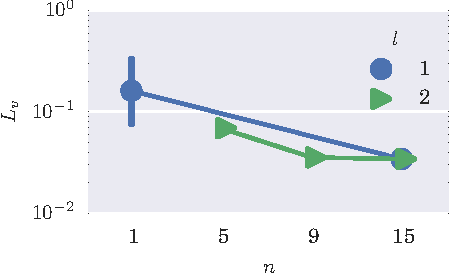
\includegraphics[width=.5\textwidth]{figs/bo_ecg.pdf}
        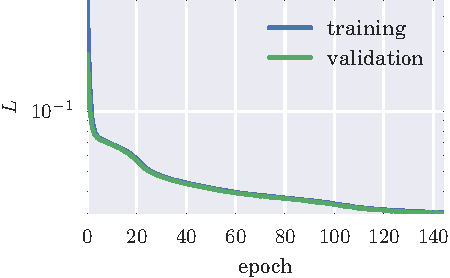
\includegraphics[width=.5\textwidth]{figs/trn_ecg.pdf}
        \caption{ECG}
    \end{subfigure}%

\end{figure}
\begin{figure}[!h] %OBVIOUSLY no p on last one...OBVIOUSLY!!
\ContinuedFloat

    \begin{subfigure}[t]{\textwidth} 
        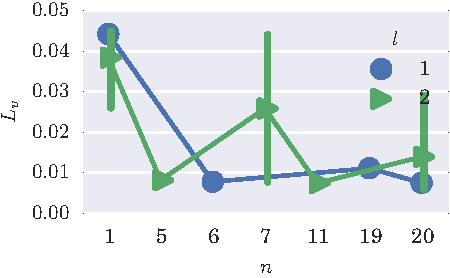
\includegraphics[width=.5\textwidth]{figs/bo_sleep.pdf}
        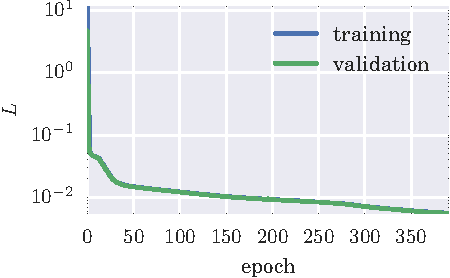
\includegraphics[width=.5\textwidth]{figs/trn_sleep.pdf}
        \caption{PSG-ECG}
    \end{subfigure}%


\caption[Training results]{Bayesian optimized validation loss (left) and training progress of best RNN (right).
%
Each point is the average validation loss since more than on training session could have been launched with the same parameters.
%
If so, the points have a 95\% confidence interval bar through them.
} 
\label{fig:bo} %OBVIOUSLY label should be AFTER caption!!!
\end{figure}
%todo: make figures centered by adding whitespace to the right



\section{Results and Discussion}
\label{sec:results}

The optimal RNN has some expectation of the typical series.
%
So, a `reconstruction error' is the difference between the test input and the output.
%
Therefore, the square of the reconstruction error can be used as an anomaly score \cite{Erfani2014}.
%
This section will show how the various calculations of error can be used to detect point anomalies \emph{as well as} discord anomalies introduced in \ref{sec:anomalytypes}.
%
However, the particular (objective) anomaly detection technique will not be discussed;
only the anomaly score, that could be used in such a technique, is presented.
%
Nonetheless, the argument is made for the ability of autoencoding RNNs to detect anomalies.


Although the order of the anomaly scores should not be important to the anomaly detection technique, sequences of error calculations can be made in two ways for a test series: 1) the MSE of a sliding window and 2) the squared error of every point in the test series where the whole sequence is input to the optimal RNN.
%
While the MSE from a sliding window can detect both point anomalies and discords, it is preferable not to have to specify a window size.
%
Ideally, high anomaly scores for points close together signal a discord while a lone high anomaly score signals a point anomaly.
%
But both types of calculations are evaluated in this discussion.


Error calculations are presented graphically in Figure \ref{fig:err} for each series (see Figure caption after the last subfigure).
%
The errors are summarized by their maximum, kernel density estimate, and the 5 percentile mark.
%
Together, with the error plot, the efficacy of the RNN in distinguishing anomalies can be evaluated;
%
normal data should correspond to the bulk of the error calculations while anomalies should correspond to extreme high values.


It should be noted that as the window size is increased, fractionally less points are included in the, normal, 95 percentile (and vice versa).
%
The kernel density estimate might change significantly accordingly.


What follows is a discussion of the ability of the (optimal) RNN to detect anomalies referencing subfigures of Figure \ref{fig:err}.


\noindent {\bfseries{spikes-1}}

\begin{figure}[!hp] %todo: i think gmu wants all figs at the top
    \centering
  
  \begin{subfigure}[t]{\textwidth}
        \centering
        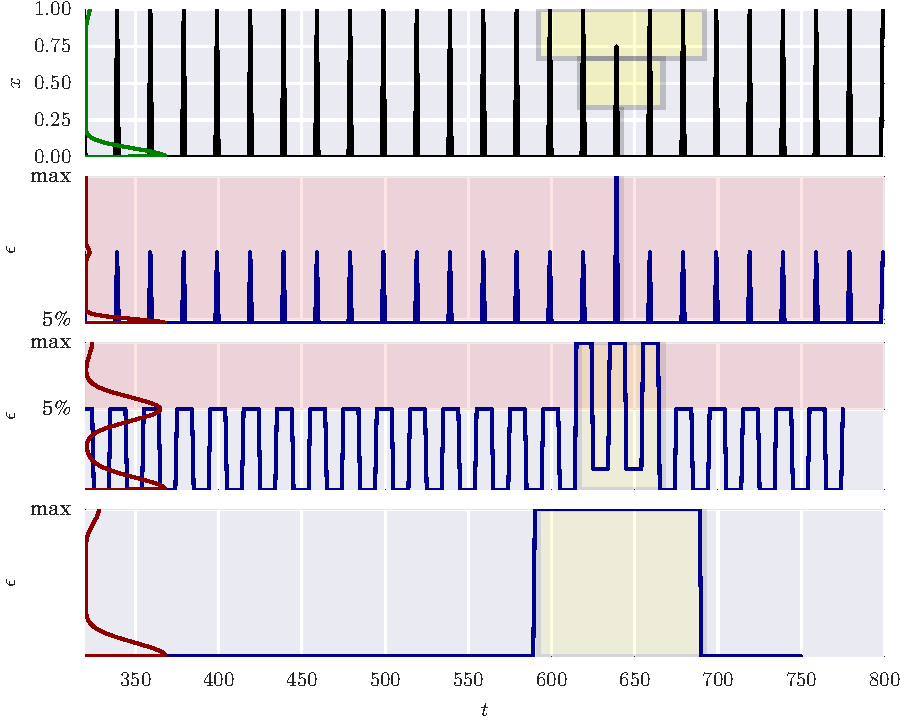
\includegraphics[]{figs/er_spikelv.pdf}
        \caption{spikes-1}
    \end{subfigure}%

\end{figure}

This series can be considered discrete with a point anomaly.
%
The point anomaly takes on an improbable value but is not extreme.
%
Clearly, the anomalies are distinguished in all error calculations.

Note the error increases as soon as the sliding window (from the left) encounters the anomaly.
%
This observation can be used to analyze the other series.


\noindent {\bfseries{spikes-2}}

\begin{figure}[!hp]
    \ContinuedFloat 
    \begin{subfigure}[t]{\textwidth}
        \centering
        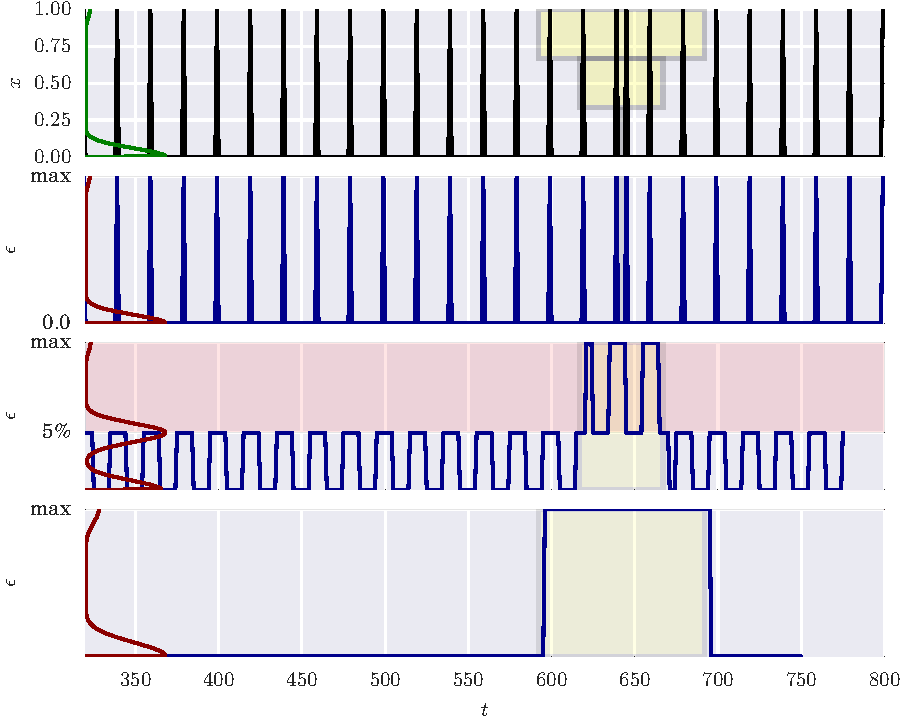
\includegraphics[]{figs/er_spikereg.pdf}
        \caption{spikes-2}
    \end{subfigure}%
\end{figure}

This spike series tests if the error becomes significant where the spike is out of place; a discord.
%
The anomaly is definitely detected in the windowed error plot but not the point error plot.


\noindent {\bfseries{sine}}


\begin{figure}[!hp]
    \ContinuedFloat 
  
    \begin{subfigure}[t]{\textwidth}
        \centering
        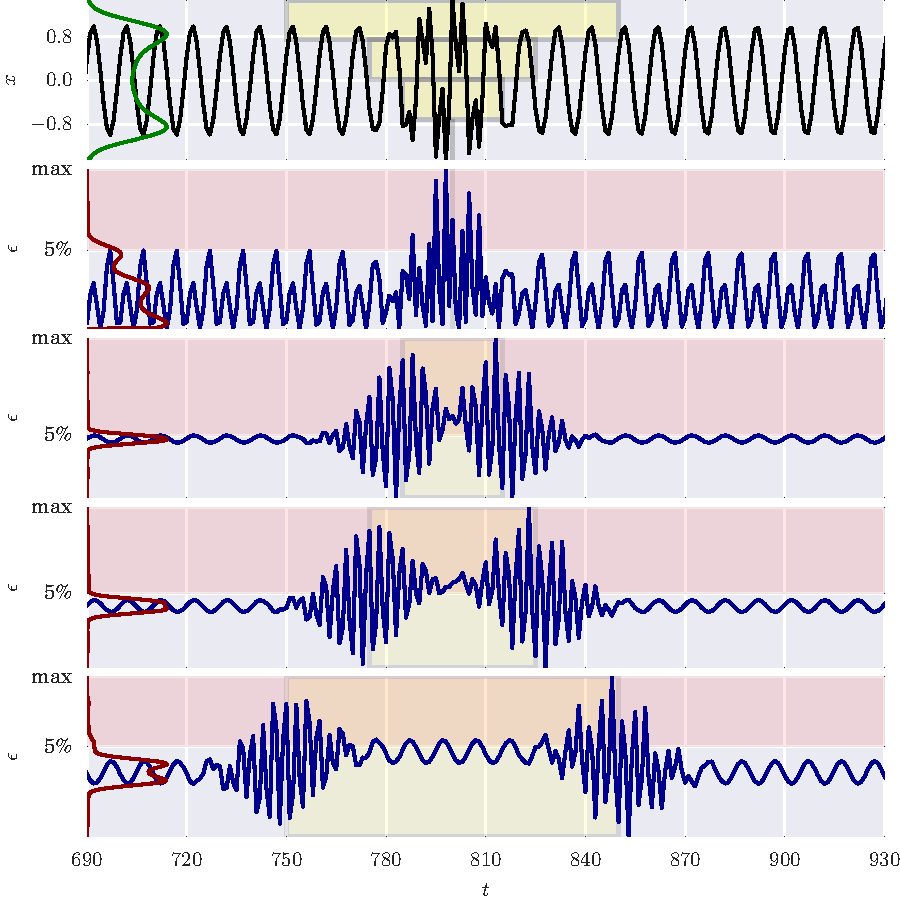
\includegraphics[]{figs/er_sin.pdf}
        \caption{sine}
    \end{subfigure}%

\end{figure}

This series tests discord because no single point is anomalous.
%
For the windowed errors, the anomalous and normal regions are distinguished by a range of values for each.
%
But, there was a transition region with errors higher or lower than the anomalous region.
%
In the point error plot, the extreme values correspond to extreme values in the test plot.
%
So, given these results, the windowed error can be more attributed to the extreme values of the test series than to its anomalous behavior.
%
In any case the RNN found a tight expectation for typical values.
%kde bad

\noindent {\bfseries{power}}

\begin{figure}[!hp]
    \ContinuedFloat 

    \begin{subfigure}[t]{\textwidth} 
        \centering
        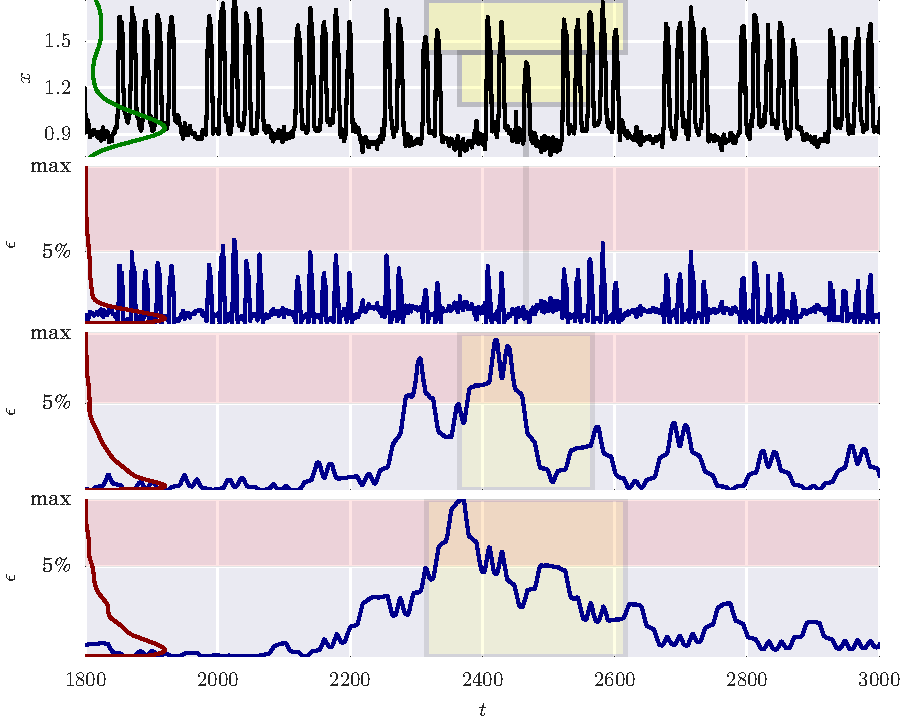
\includegraphics[]{figs/er_power.pdf}
        \caption{power}
    \end{subfigure}%

\end{figure}

The power series normally shows a demand profile over a five-day work week.
%
The windowed error distribution has a long tail because high errors were given to normal areas of test series (not shown within the plot, possibly due to some drift in the series).
%
In fact, the first windowed error plot does not contain the highest error unlike the second windowed error plot.
%
Nonetheless, both windowed errors distinguished the anomalous region.
%
But, obviously, the point errors can not be used to detect the anomalous region.


\noindent {\bfseries{ECG}}

\begin{figure}[!hp]
    \ContinuedFloat 

    \begin{subfigure}[t]{\textwidth} 
        \centering
        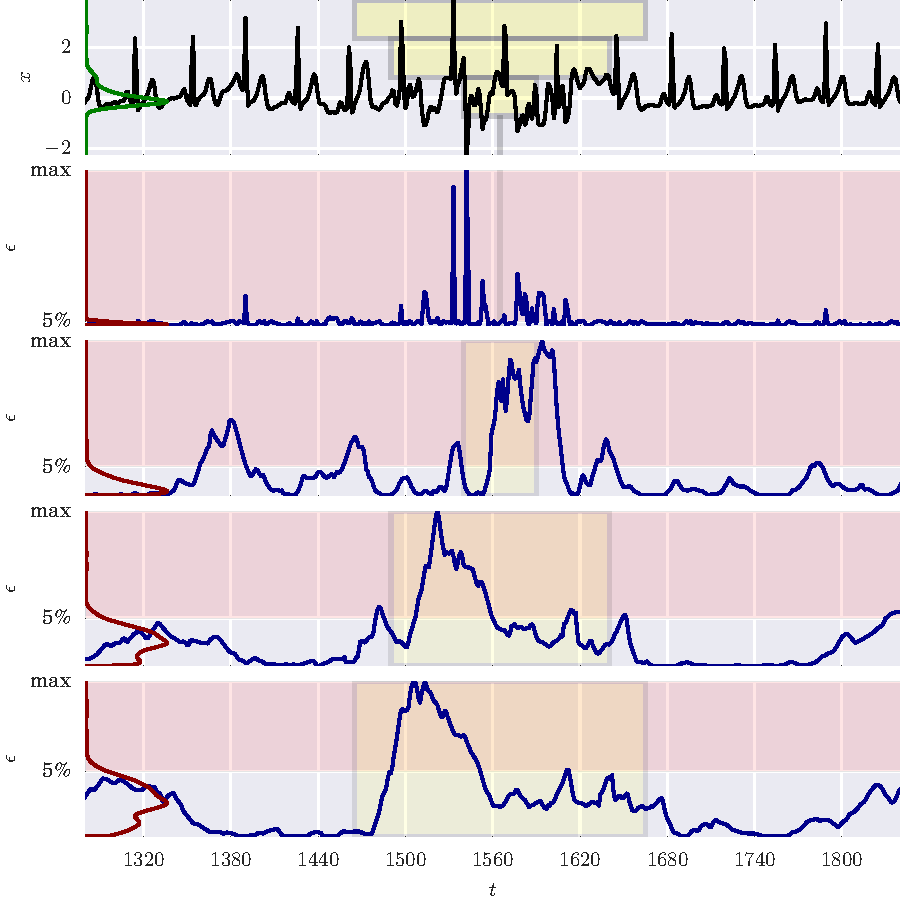
\includegraphics[]{figs/er_ecg.pdf}
        \caption{ECG}
    \end{subfigure}%

\end{figure}


The ECG is a challenging series because, while there is a repeating element, the element does not precisely have the same period.
%
There is also noise in the signal that has to be distinguished from its significant features.

In the point error plot, the most prominent values correspond to points on the test series that are simply lower than a baseline.
%
The same cannot be said about the error plot with the smallest window;
%
although the areas with extreme values are the most prominent, areas that have different behavior, but not extreme in value, are distinguished as well.
%
For example, a particularly subtle anomaly was detected within the highest 5 percentile at around $t=1380$ despite the fact that the more anomalous \emph{region} contributed extreme values.
%
The same could be said about anomaly at around $t=1470$.
%
This window size was chosen to be about the size of the repeating unit since the effect of these anomalies on the error is diluted for larger windows.
%
%Still, an argument can be made that the larger windows captured the anomalous region's behavior, as opposed to just its extreme values, because a significant portion of the error corresponding to the anomalous region lies within the 95 percentile (and hence within the normal range of error fluctuations for normal data). %weak :S
The larger windows detected the most anomalous region but it is not apparent whether the extreme error values were due to deviant values or deviant behavior.


\noindent {\bfseries{PSG-ECG}}

In this ECG, the point errors do not reveal much about the anomalous region because every spike in the error plot plot corresponds to a normal spike in the ECG, normal or otherwise.
%
However, the anomalous region is clearly detected in both windowed error plots.
%
Again the error in the anomalous region is well beyond the normal range of error fluctuations albeit the test series values are slightly above average (as can be seen from the density estimate).

\begin{figure}[!hp] 
    \ContinuedFloat

    \begin{subfigure}[t]{\textwidth} 
        \centering
        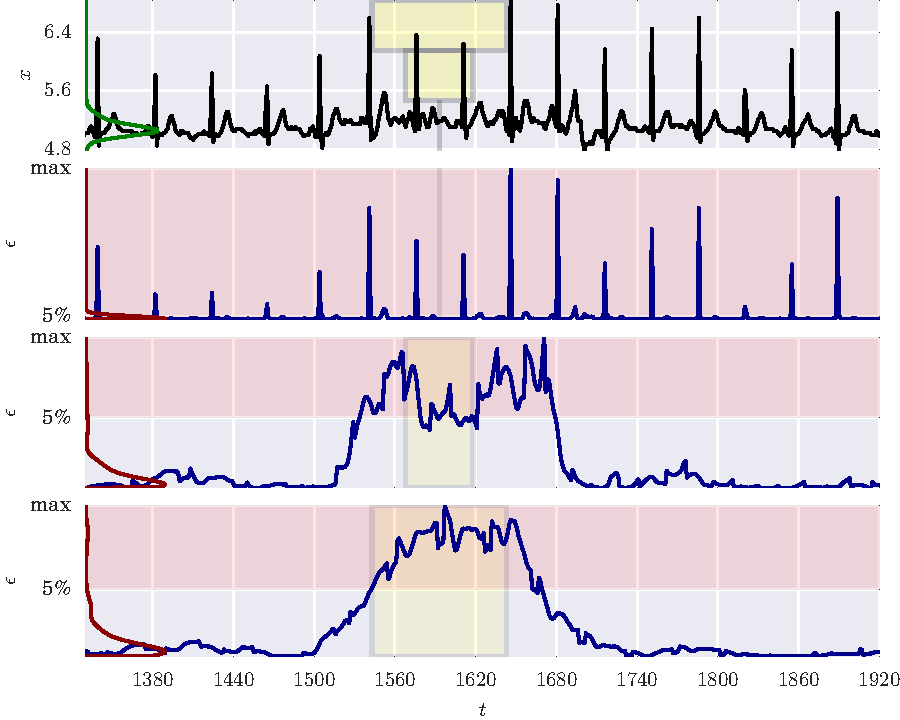
\includegraphics[]{figs/er_sleep.pdf}
        \caption{PSG-ECG}
    \end{subfigure}%

\caption[Anomaly scores of series]{Anomaly scores of series.
%
In the top pane, a portion of the input series is shown with an anomaly.
%
While the focus is on the anomaly, enough normal data is shown for subjective comparison.
%
This is accompanied by a kernel density estimate, plotted on the ordinate (vertically), to evaluate the normality of the data \emph{by value} as opposed to \emph{behavior}.
%
The lower panes show series of squared error, $\epsilon$, where each pane is associated with a sliding window size.
%
The window size is represented by a highlighted vertical span in the error plot as well as a corresponding box in the input series plot to give a sense of scale to the anomaly relative to the window.
%
Sliding a window over the test series that calculates its MSE generates the error series (error calculation type 1).
%
The locations of the MSE points correspond with the center of the sliding window.
%
However, error plots with just a vertical line as a `window' are just individual squared errors (error calculation type 2).
%
Furthermore, a kernel density estimate for all the errors (including ones outside the plot) is plotted (vertically) on the ordinate.
%
The highest 5 percentile and the maximum of (all) the errors are marked on the ordinate also.
}
\label{fig:err}
\end{figure}

%todo:replace: indices to ^X^X FOR p omitted
%todo: 'was programmed to save'  ...just write: process saves
\section{Conclusions}

Given the results, which are influenced by the described training process and RNN architecture, some general statements can be made about how well the RNNs can find anomalies.

\begin{itemize}

\item 
  Using the point errors, extreme, but not necessarily rare, values can be found.

\item
  The windowed errors are a versatile way of finding, both point and discord, anomalies at multiple scales.
  % 
  However, this means that the window size must be about the same scale as the anomaly.
  % 
  Else, the effect of the anomaly would not be pronounced.
  %
  Furthermore, the minimum window size must be long enough to contain meaningful dynamics.

\item
  Pursuant to the previous two points, windowed errors are more reliable in finding anomalies.

\item
  The training data can have some anomalous data.

\item
  The RNNs were insensitive to variations in sequence length and translation.

\item
  With minor variation, the same process can be used to find anomalies in a variety of series.

\end{itemize}

In general, subject to effective training, the RNNs `learned' the typical \emph{behavior} of the series which includes information about their typical values as well as their ordering.
%
Concludingly, the autoencoding recurrent neural network can be used to detect anomalies in sequences.


%todo . theano implememtation particularly slow suspected
%todo. include tbls and probabilitydfs in repo in final

%%% Local Variables:
%%% mode: latex
%%% TeX-command-extra-options: "-shell-escape"
%%% TeX-master: "thesis"
%%% End:
